En este capítulo se desarrollan en detalle todos los procesos que se llevan a cabo en la sección administrativa del centro.

\section{Distribución de la plantilla}

El equipo administrativo del centro de salud está compuesto por siete miembros. En la Figura~\ref{fig:plano-interior} se muestra la posición de cada unos de los puestos.

\begin{itemize}
    \item Puestos de ventanilla: 1, 2, 3 y 4
    \item Puestos de interior: 5 y 6
    \item Jefe de grupo: 7
\end{itemize}

\begin{figure}[H]
    \centering
    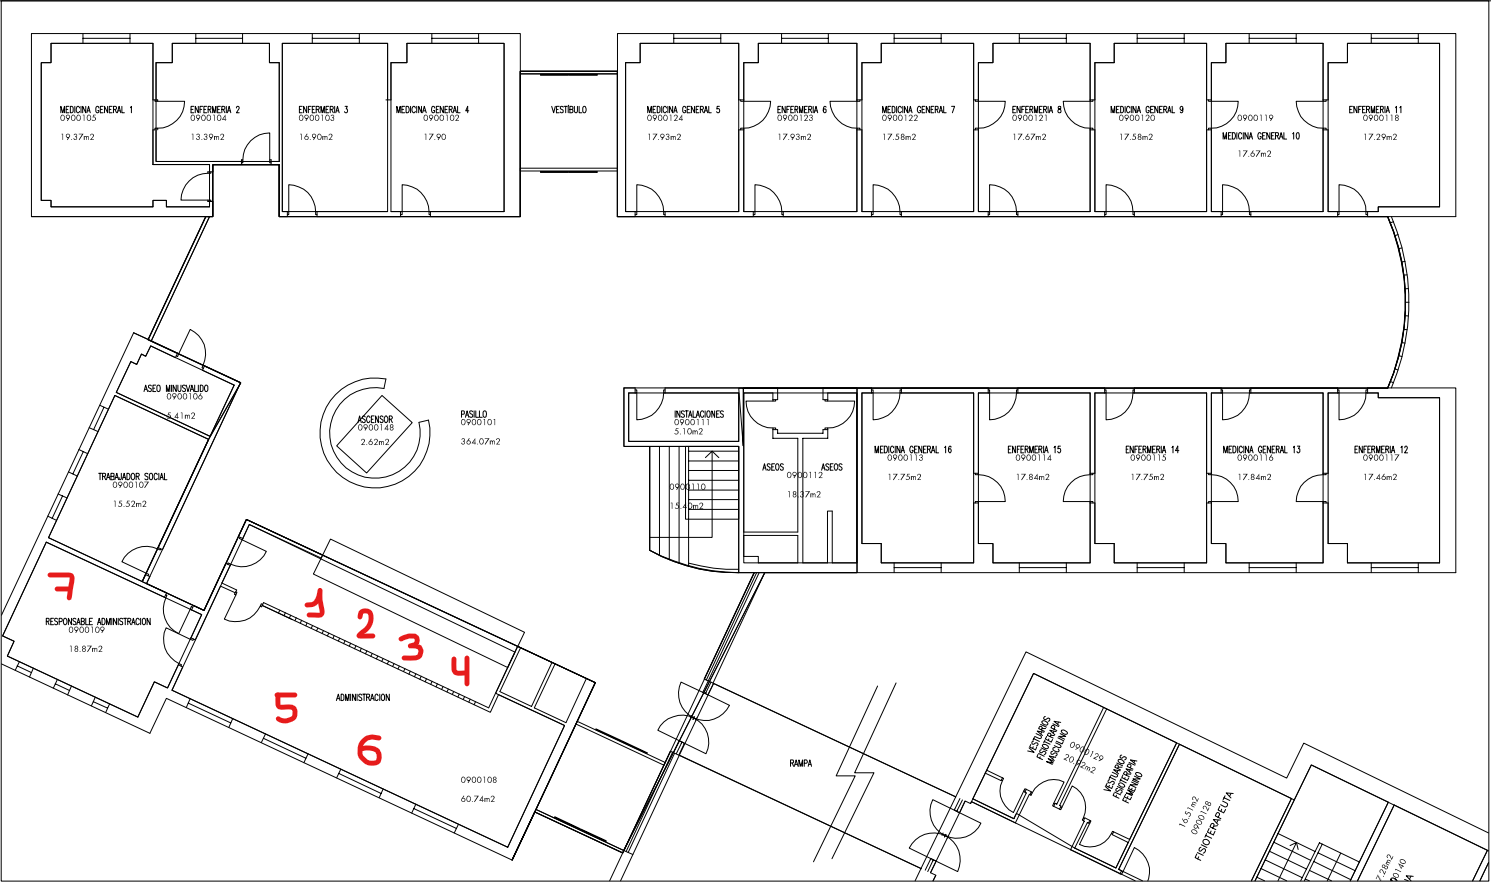
\includegraphics[width=\textwidth]{img/plano-interior.png}
    \caption{Distribución de la planta baja del centro de salud}
    \label{fig:plano-interior}
\end{figure}

\section{Procesos administrativos}

En este apartado se describen los distintos procesos que existen en la sección administrativa.
Para cada proceso existe al menos un diagrama BPMN, incluidos en el anexo de este trabajo, que describe de una manera visual el flujo de información que sucede en cada proceso.

\subsection{Gestión de citas previas}

Un paciente puede solicitar una cita con un profesional sanitario de atención primaria por dos vías: en el propio centro de salud o a través de la aplicación de \Gls{sacyl-conecta}.
Si el usuario decide solicitar cita previa vía online la realización de la tarea es diferida, es decir, no tiene por qué realizarse en el momento.
De esta forma, al final de la jornada o cuando el trabajo lo permita, se revisan las peticiones de citas y se tramitan en el programa \Gls{medora}.
Por el contrario, si el usuario acude al centro de salud (ver diagrama de proceso en la Figura~\ref{fig:proceso-consultas} y lista de tareas en la Tabla~\ref{tab:proceso-consultas}), la cita se programa en el momento, entregando un justificante en papel.
Todas las citas se programan a través de \Gls{medora} aunque hay algunas diferencias dependiendo del profesional al que vaya destinado.

\begin{table}[H]
    \begin{tabular}{lp{5cm}llll}
        \toprule
        Código & Tarea                   & Puesto     & Demandante & Programa & Carga \\
        \midrule
        CO01   & Identificar al paciente & Ventanilla & Paciente   & Tarjeta  & Baja  \\
        CO02   & Dar cita previa         & Ventanilla & Paciente   & Tarjeta  & Media \\
        CO03   & Imprimir pegatinas      & Ventanilla & Paciente   & Tarjeta  & Alta  \\
        CO04   & Imprimir citas previas  & Ventanilla & Paciente   & Tarjeta  & Baja  \\
        \bottomrule
    \end{tabular}
    \caption{Listado de tareas para el proceso de gestión de tarjeta sanitaria}
    \label{tab:proceso-consultas}
\end{table}

\subsubsection{Citas generales}

Las \textbf{consultas de medicina familiar} se citan en los huecos\footnote{Se refiere a la franja de tiempo que se reserva para cada tipo de consulta.} de demanda.
Sin embargo, si se trata de un parte de \gls{incapacidad-temporal} o una receta médica se citan en los huecos de consulta administrativa.
Por lo general no se cita en otros huecos a excepción de si es un aviso, que se cita en domicilio.
En este último caso siempre se debe confirmar la dirección del domicilio y el teléfono del paciente.
En el caso de que sea un aviso urgente, se llama al médico para que el paciente o el familiar le explique el estado.
El médico entonces valora si necesita atención urgente o no.
También es importante asegurarse que el paciente identificado es al que realmente se quiere dar una cita ya que puede haber confusión con pacientes de igual nombre y apellidos.
Para evitar esta situación se debe de verificar la fecha de nacimiento con el documento de identidad.

Por lo general, las \textbf{citas de enfermería} se citan a demanda.
También existe la posibilidad de poner un aviso a domicilio asegurándose siempre de confirmar la fecha de la cita, el domicilio del pacientes y su número de teléfono.
Además, se debe especificar el motivo de la consulta: curas, sondas, extracciones, etc.
En el caso de que haya que realizar una analítica se debe de fotocopiar el \gls{volante}.
Los \glspl{electrocardiograma} se citan con el enfermero correspondiente reservando dos huecos de la agenda ya que son pruebas más largas.
Las consultas de enfermería pediátrica se citan según el calendario del programa del niño sano\footnote{Actuaciones preventivas y de promoción de la salud, que se llevan a cabo periódicamente con el fin de controlar que el niño se está desarrollando y creciendo de manera correcta.}, en los huecos de programada o demanda según corresponda. Si es necesario conviene hablar con los profesionales.

Las \textbf{citas pediátricas} se citan en los huecos de demanda de la agenda si es una consulta normal.
Las consultas programadas se citan en los huecos correspondientes según el calendario de revisiones del niño sano, procurando que aquellas que corresponden a pediatra y a enfermera coincidan en el mismo día.
Los huecos RN se deben de asignar a las revisiones de neonatos entre los cinco y siete días de vida.
Las urgencias pediátricas se citan en los huecos de enfermería forzando, si es necesario, la cita.
Si la enfermera que corresponde al paciente no se encuentra disponible, se asigna la cita con otra enfermera.
En el caso de niños desplazados\footnote{Pacientes que se han cambiado de residencia por un periodo inferior a tres meses} o transeúntes\footnote{Igual que los desplazados pero con una estancia inferior a un mes} que deban ser citados de urgencia, se les asignará el pediatra que asuma ese día la \gls{guardia}.

Existen distintos tipos de \textbf{consulta de obstetrcia}.
En lo posible, hay que respetar cada tramo aunque, si es necesario, conviene hablar con la \gls{matrona} en caso de duda.

Las \textbf{consultas con el trabajador social} solamente son tres días a la semana: lunes, martes y miércoles.
Solo es posible citar en los huecos de demanda.

\subsubsection{Citas de especialidades}

Para citar consultas de especialidades es imprescindible que el paciente presente la tarjeta sanitaria.
La excepción es cuando el paciente trae una hoja de citación en la que figura el número de historia clínica, el NHC.
Igualmente, es imprescindible un \gls{volante} de petición de un facultativo.
Es importante comprobar que la tarjeta que entrega el paciente se corresponde con la persona que se indica en el \gls{volante}.
Se vuelcan los datos de la tarjeta sanitaria en el programa y se verifica la dirección del domicilio y el teléfono. De lo contrario, no se puede dar la cita.
La identificación del paciente se puede hacer, si no funciona con la tarjeta, por número de afiliación junto con los apellidos, nombre, fecha de nacimiento, documento de identidad o cualquier otro campo.
Tras la identificación, se pincha en la tarjeta sanitaria para proceder a la comprobación y volcado de todos los datos.
Si los datos no son correctos, se modifican en el programa de \Gls{tarjeta-sanitaria}.
A continuación, en el puesto de citación, se comprueba nuevamente que la persona que aparece en pantalla es a la que realmente queremos citar.
De la misma forma, hay que tener especial cuidado a la hora de entregar la hoja de cita del paciente.

Ante un \gls{volante} de cirugía vascular, pediátrica o torácica, se cita la consulta de la especialidad concreta en \Gls{medora}.
Se pincha en el primer hueco disponible anotando la fecha de la cita del \gls{volante} y se guarda en la carpeta ``Hospital Clínico''.
Diariamente, se imprime la agenda de cada día desde \Gls{medora} y se envía vía fax junto con los volantes.
Cuando se reciben las citas, también vía fax, se espera a recibir la nota de citación.
Esta se envía al paciente haciéndolo constar previamente en la hoja que archiva en el centro.

Las \textbf{citas de radiología} se solicitan en ventanilla y con el \gls{volante}.
Se debe de indicar en el \gls{volante} el número de historia clínica antes de imprimir la cita.
Este proceso se puede realizar también por vía telefónica.
Las radiografías que no se pueden hacer en el centro de salud son las columnas totales y otras más específicas que se realizan en el Centro de Especialidades Arturo Eyries.
Las ecografías se citan también en el Hospital.

Por otro lado, las \textbf{citas de ginecología} solo se pueden dar para los ginecólogos del propio centro de salud.
Los pacientes que deseen otro ginecólogo o en otro centro, deberán redactar un escrito y presentarlo en la sección de Atención al Paciente del Hospital Río Hortega.

Las \textbf{consultas de odontología} se citan en la agenda correspondiente de \Gls{medora}.
El dentista suele pedir \gls{ortopantomografías} mediante \gls{volante}.
Este tipo de prueba radiológica se realiza en el Hospital Río Hortega solicitando previamente cita.
Es importante citar al paciente al día siguiente de la radiografía para que el odontólogo vea los resultados.

\subsubsection{Laboratorio}

Las extracciones de sangre se citan en los huecos de agenda con el mismo nombre.
En caso de que haya sido solicitada por un especialista, se debe de indicar específicamente dado que no necesita pegatina.
De la misma forma, se debe de anotar los tres últimos dígitos del número de petición en las que son solicitadas por el médico de familia.

Diariamente, se sacarán las pegatinas correspondientes al día siguiente para el laboratorio.
Para ello, primero hay que imprimir el listado por orden alfabético de los apellidos desde el programa \Gls{medora}.
Una vez obtenidas todas las pegatinas, es necesario comprobar que han salido todas y están correctamente impresas.

% \subsubsection{Citas preferentes}

% Las citas preferentes que paute el profesional médico se tramitan desde el puesto de ventanilla en la consulta virtual habilitada para tal efecto.
% En este caso no se imprime la hoja de cita pero la primera hoja del \gls{volante} se guardará en el archivador correspondiente ``Preferentes pendientes'' por orden alfabético del puesto interior.

% Las ecografías preferentes o de la unidad de mamografías, se envían por fax a Lourdes.
% Los \gls{nodulos-tiroideos} tendrán la misma consideración.

% Cuando se reciban las citas, se debe hacer constar en la copia enviada, la fecha de recepción de la cita y la tramitación que se hace de ella.
% Si la cita es muy inmediata y no da tiempo a enviar el correo, se deja en ventanilla.
% En este último caso, se llama al paciente por teléfono para comunicarle la cita y se le indica que debe pasar por ventanilla del centro de salud para recoger su citación.
% Posteriormente, el documento se mueve del archivador ``Citas pendientes'' al archivador ``Resueltos''.

% Cuando se reciben las citas desde la Gerencia, se comprueban que llegan todas las que se enviaron. En caso de no haber recibido alguna, se debe reclamar a la misma Gerencia.

% \subsubsection{Consultas simtron}

% Desde septiembre de 2016, se citan en la consulta de enfermería desde \Gls{medora}.
% A excepción de los pacientes procedentes de residencias geriátricas, que se citan en el puesto interior de laboratorio.
% Una vez se reciben los resultados del control de \Gls{sintrom}, se envían por fax a las distintas residencias geriátricas.

% Del mismo modo, enfermería se encargará de obtener e imprimir los resultados de la prueba en el puesto interior.

% En algunas ocasiones, a primera hora de la mañana una de las residencias envía vía fax la nota de \Gls{sintrom} de alguno de los pacientes.
% En este caso, se citará en el mismo día en la consulta de enfermería y se colocará el documento en el casillero correspondiente al enfermero.

\subsection{Tarjeta sanitaria}

En muchas ocasiones, un paciente acude al centro de salud no por necesitar atención sanitaria sino por motivos administrativos: alta en el sistema de salud, actualización de datos personales de la tarjeta o incluso un cambio de médico de familia. Para todos estos casos, existe un programa informático llamado \Gls{tarjeta-sanitaria} donde se registran todos estos trámites. El diagrama del proceso se expone en la Figura~\ref{fig:proceso-tarjeta} y el listado de tareas en la Tabla~\ref{tab:proceso-tarjeta}.

\begin{table}[H]
    \begin{tabular}{lp{5cm}llll}
        \toprule
        Código & Tarea                                 & Puesto     & Demandante & Programa & Carga \\
        \midrule
        TA01   & Crear nueva tarjeta                   & Ventanilla & Paciente   & Tarjeta  & Alta  \\
        TA02   & Actualizar datos de tarjeta sanitaria & Ventanilla & Paciente   & Tarjeta  & Media \\
        TA03   & Recuperar tarjeta                     & Ventanilla & Paciente   & Tarjeta  & Media \\
        TA04   & Crear tarjeta temporal                & Ventanilla & Paciente   & Tarjeta  & Media \\
        \bottomrule
    \end{tabular}
    \caption{Listado de tareas para el proceso de gestión de tarjeta sanitaria}
    \label{tab:proceso-tarjeta}
\end{table}

\subsubsection{Paciente nuevo}

En el caso de un paciente nuevo o de un recién nacido, se añade en el programa introduciendo previamente el número del documento de identidad o el número de afiliación a la seguridad social.
A continuación, el paciente aparecerá en la base de datos de la comunidad o en la de la Seguridad Social.
Se rellenan todos los campos necesarios y se imprime el documento justificativo con el sello del centro.

\subsubsection{Modificación de datos}

Para realizar un cambio de domicilio, de número de teléfono, error en los datos de la tarjeta o la inclusión del número del documento de identidad.

Primeramente, se debe confirmar que el paciente existe en la base de datos de \Gls{tarjeta-sanitaria}.
Si es así, se confirman o se modifican los datos que correspondan.
Si se da el caso de que el paciente esté dado de baja en el sistema, se le recupera.

El modo más rápido de identificación de un paciente es través de su documento de identidad o el número de afiliación de asistencia.
También cabe la posibilidad de que sea un alta nueva o un cambio de domicilio, de Gerencia o incluso la emisión de una tarjeta de desplazado.

Los mayores de catorce años, además de la inclusión del documento de identidad, se les asignará el médico de familia que tenga el titular.
Como motivo de modificación se consignará el paso de oficio de pediatra a médico general.
Finalmente se imprime el documento y se sella.

\subsubsection{Extravío o deterioro}

Se identifica al paciente en la primera pantalla del programa.
A continuación, en la pestaña de tarjetas, se localiza y se indica si es un extravío o un deterioro.
Se imprime el documento y se sella.

\subsubsection{Desplazados-transeúntes}

Un paciente puede solicitar un desplazamiento con una duración máxima de tres meses que puede ser prorrogado otros tres.
Posteriormente, habría que darlo de alta en el sistema.

Primero, se identifica al paciente, se modifica y se emite la cartulina de desplazado.
Se cumplimentan todos los datos, indicando específicamente en la pantalla inicial que es un desplazamiento.
Se rellenan los datos relativos a la dirección del domicilio y el número de teléfono.

En cuanto a la asignación del médico, si viven con un familiar en el mismo domicilio, se le asignará el médico de familia.
De lo contrario, se le asigna al médico que tenga el cupo abierto.

Finalmente, se imprimr el documento justificativo y se sella.
Se debe de indicar en este momento la fecha de validez del desplazamiento.
Igualmente, se debe de comunicar al paciente que para recibir asistencia sanitaria es preciso presentar tanto la tarjeta sanitaria personal como el documento de desplazamiento.

Cuando el periodo de permanencia es muy corto, inferior a un mes.
Se procede del mismo modo que los desplazamientos pero especificando en el programa que es del tipo ``Transeúnte''.

\subsection{Gestión de personal: Agendas}

La gestión de agendas recoge todas la tareas  relacionadas con la asignación de franjas de tiempo, o huecos, a los distintos profesionales y sus respectivas modificaciones. En la Tabla~\ref{tab:proceso-agendas} se muestra un listado de las tareas pertenecientes a este proceso. Además, en el diagrama BPMN expuesto en la Figura~\ref{fig:proceso-agendas} se puede observar el flujo que se sigue a día de hoy.

\begin{table}[H]
    \begin{tabular}{lp{5cm}llll}
        \toprule
        Código & Tarea                                & Puesto   & Demandante & Programa & Carga \\
        \midrule
        AG01   & Alta a nuevos profesionales          & Interior & Personal   & Medora   & Media \\
        AG02   & Transferir citas entre profesionales & Interior & Personal   & Medora   & Baja  \\
        AG03   & Realizar sustituciones               & Interior & Personal   & Medora   & Media \\
        AG04   & Realizar autorizaciones              & Interior & Personal   & Medora   & Media \\
        \bottomrule
    \end{tabular}
    \caption{Listado de tareas para el proceso de gestión de agendas}
    \label{tab:proceso-agendas}
\end{table}

Todas las tareas relacionadas con la agenda comienza con la búsqueda de los trabajadores en el programa \Gls{medora} seleccionando la categoría y especificando el nombre del profesional u otros datos.
Es importante pinchar en la pestaña de ``todos'' antes de buscar al profesional.
Se muestran todos los datos e información de la plaza del profesional además del Código de Identificación Autonómica Sanitaria\footnote{Número que identifica a un profesional médico.} o si es sustituto.

Para dar de alta un trabajador o crear una sustitución primero es necesario comprobar si ya existe en la base de datos.
Si el profesional ya ha estado previamente en el centro de salud de Laguna de Duero, hay que recuperarle ya que aparecería de color naranja en el programa.
En la pestaña de ``Modificar'' se pasa a ``Activo'' para poder realizar la sustución u otro tipo de modificación.
Si, por el contrario, el profesional no ha estado nunca en el centro de salud de Laguna habría que acceder a la pestaña de gestión de sustituciones y ver qué profesional falta y quién le sustituye.

Para crear una sustitución o dar de alta, se rellenan los campos de la pestaña de Gestión de Sustituciones especificando el profesional que sustituye junto con el día y la hora. En caso de que no sea posible realizar la sustitución, se realiza una autorización siguiendo el mismo procedimiento.

Para transferir las citas del profesional ausente se bloquea la agenda de Medora del que falta indicando la fecha y la hora de las citas.

\subsection{Cargos a terceros}

Por lo general, los pacientes que acuden al centro de salud tienen acceso gratuito a la cartera de servicios de Atención Primaria, sin embargo, hay ciertos casos en los que el Sistema Público de Salud no asume el coste y que por tanto se debe de cobrar al paciente. Las tareas se listan en la Tabla~\ref{tab:proceso-cargos} y en el diagrama de la Figura~\ref{fig:proceso-cargos}.

\begin{table}[H]
    \begin{tabular}{lp{5cm}llll}
        \toprule
        Código & Tarea                                & Puesto     & Demandante & Programa & Carga \\
        \midrule
        CA01   & Identificar al paciente              & Ventanilla & Paciente   & -        & Baja  \\
        CA02   & Recepcionar fotocopias               & Ventanilla & Paciente   & -        & Baja  \\
        CA03   & Informar al paciente de los trámites & Ventanilla & Paciente   & -        & Baja  \\
        CA04   & Solicitar documentos específicos     & Ventanilla & Paciente   & -        & Baja  \\
        CA05   & Enviar documentación a la Gerencia   & Interior   & Gerencia   & -        & Baja  \\
        \bottomrule
    \end{tabular}
    \caption{Listado de tareas para el proceso de gestión de cargos a terceros}
    \label{tab:proceso-cargos}
\end{table}

\subsubsection{Convenios internacionales}

En este caso de debe rellenar el formulario \textit{H-111}, indicando diagnóstico, fecha de asistencia y firma del paciente.
Es muy importante presentar una fotocopia de la tarjeta sanitaria europea o un documento equivalente.

En el caso de que no se presente, se debe anotar el número de teléfono y el correo electrónico para poder contactar con el paciente desde la sección de ``Cargos a terceros'' del Hospital Universitario Rio Hortega.

También es necesario que el paciente firme la nota informativa ya que es el documento requerido para la protección de datos y el compromiso de hacerse cargo del importe del gasto.

\subsubsection{Accidentes de tráfico}

En el caso de un accidente de tráfico es necesario que el paciente rellene la ficha de asistencia sanitaria, firme la nota informativa y complete la solicitud de datos de accidente de tráfico.
Este último documento debe concordar con los datos presentes en el atestado\footnote{Documento oficial que elabora la Guardia Civil o una entidad policial local, en el que se describen los detalles de un accidente de tráfico} del accidente.

\subsubsection{Accidentes de trabajo}

En este caso tan solo es necesario rellenar la ficha de asistencia sanitaria y firmar la nota informativa.

\subsubsection{Espectáculos taurinos}

Se rellena la ficha de asistencia sanitaria junto con la firma de la nota interior.
En este caso, se debe de completar el documento ``Lesionados en espectáculos taurinos'' especificando el lugar donde se realiza el espectáculo y quién es el responsable del mismo (Ayuntamiento, asociaciones taurinas, etc).

\subsubsection{Agresiones}

En este caso tan solo es necesario rellenar la ficha de asistencia sanitaria y firmar la nota informativa.

\subsubsection{Accidentes deportivos o de caza}

Además de la ficha de asistencia sanitaria y la nota informativa, el paciente debe presentar una fotocopia de su licencia federativa junto con la información del seguro que cubre el siniestro, especificando el número de póliza y el número de siniestro.

\subsubsection{Seguros privados}

Se rellena la ficha de asistencia sanitaria junto con la firma de la nota informativa.
Se debe presentar también una copia del parte de accidente, la petición de asistencia o cualquier otro documento de acepctación del gasto que haya sido expedido por la empresa, la compañía de seguros o la mutua.
En el caso de que sea un paciente desplazado, se debe presentar la fotocopia de la tarjeta de mutualista.

\subsubsection{Particulares}

Se completa la ficha de asistencia sanitaria y se firma la nota informativa.
Este último documento es muy importante ya que hace constar que el paciente se responsabiliza del importe del cargo.

\subsection{Reclamaciones}

El proceso de reclamaciones se inicia, generalmente, cuando un usuario se acerca a la ventanilla de admisión solicitando poner una reclamación.
En el listado de tareas de la Tabla~\ref{tab:proceso-reclamaciones} y en el diagrama de la Figura~\ref{fig:proceso-reclamaciones} se puede ver el proceso completo.
El usuario deberá identificarse con su documento de identidad y el personal administrativo cumplimentará la hoja de reclamación a tal efecto.
Una vez tomados los datos, el administrativo entrega al usuario la correspondiente hoja de reclamaciones para que la rellene con su demanda.
Una vez entregada la hoja de vuelta por el usuario, se registra de entrada y se entrega la hoja amarilla al paciente mientras que las dos hojas restantes se quedan en administración.

\begin{table}[H]
    \begin{tabular}{lp{5cm}llll}
        \toprule
        Código & Tarea                               & Puesto   & Demandante & Programa & Carga \\
        \midrule
        RE01   & Identificar al reclamador           & Interior & Paciente   & -        & Baja  \\
        RE02   & Entregar formulario de reclamación  & Interior & Paciente   & -        & Baja  \\
        RE03   & Entregar reclamación al responsable & Interior & Personal   & -        & Media \\
        RE04   & Enviar reclamación a la Gerencia    & Interior & Gerencia   & -        & Baja  \\
        RE05   & Archivar reclamación en el archivo  & Interior & Personal   & -        & Baja  \\
        \bottomrule
    \end{tabular}
    \caption{Listado de tareas para el proceso de gestión de reclamaciones}
    \label{tab:proceso-reclamaciones}
\end{table}

Tras esta primera fase, si el objeto de la reclamación está relacionado con un trámite administrativo es el propio jefe de grupo quien contesta la reclamación.
Si no es el caso, es el propio jefe de grupo quien entrega la reclamación al responsable correspondiente.

Una vez la reclamación ha sido contestada por el responsable, se envía una de las hojas a la Gerencia de Atención Primaria a través de correo físico ya que son ellos quienes se encargan de resolver formalmente la reclamación y hacérsela llegar al usuario a su domicilio.

Cuando la Gerencia de Atención Primaria resuelve una reclamación, además de enviar la resolución al usuario, se envía una copia al centro de salud donde se interpuso la demanda para que tengan constancia de que fue resuelta en tiempo y forma.
Este último paso es importante ya que hay casos en que los usuarios acuden al centro de salud preguntando por el estado de su reclamación.

\subsection{Permisos retribuidos}

La gestión de permisos retribuidos de los profesionales del centro de salud también recae en la sección administrativa, concretamente las tareas especificadas en la Tabla~\ref{tab:proceso-permisos} y en el diagrama de proceso de la Figura~\ref{fig:proceso-permisos}).

Cuando un profesional quiere solicitar un permiso retribuido, debe completar la petición correspondiente.
Tras completar la petición se debe entregar al responsable, en el caso de médico se entrega al coordinador del centro, para recibir la aprobación.
Si el profesional es médico, por lo general, se deja la petición en el casillero habilitado del coordinador para que lo recoja en cuanto pueda.

\begin{table}[H]
    \begin{tabular}{lp{5cm}llll}
        \toprule
        Código & Tarea                                              & Puesto   & Demandante & Programa & Carga \\
        \midrule
        PE01   & Archivar solicitud en el casillero del responsable & Interior & Paciente   & -        & Baja  \\
        PE02   & Enviar solicitud a la Gerencia                     & Interior & Gerencia   & -        & Baja  \\
        PE03   & Guardar copia en el archivo de solicitudes         & Interior & Paciente   & -        & Baja  \\
        PE04   & Avisar al solicitante                              & Interior & Paciente   & -        & Baja  \\
        \bottomrule
    \end{tabular}
    \caption{Listado de tareas para el proceso de solicitud de permisos retribuidos}
    \label{tab:proceso-permisos}
\end{table}

Tras la aprobación del responsable, es el administrativo quien se encarga de ensobrar la petición y enviarla por correo físico a la Gerencia de Atención Primaria para su autorización.
Siempre se debe de adjuntar el original con las dos firmas, la del responsable y la del solicitante.
Se espera a recibir de vuelta la petición autorizada por la Gerencia y se realiza una fotocopia.
El original se entrega al profesional mientras que la fotocopia se guarda en la carpeta administrativa del mismo profesional, en la parte delantera de la ficha.

Cabe destacar en este proceoso que en numerosas ocasiones, debido a la lentitud del proceso provocada por el movimiento físico de papeles por correo, se da la situación de que el profesional disfruta del permiso antes, incluso, de recibir la autorización desde la Gerencia.

\subsection{Tareas generales}

En este apartado se desarrollan las tareas que no se pueden incluir en ninguno de los procesos anteriores.

\begin{table}[H]
    \begin{tabular}{lp{5cm}llll}
        \toprule
        Código & Tarea                                      & Puesto     & Demandante & Programa & Carga \\
        \midrule
        GE01   & Diseñar cartelería                         & Interior   & Paciente   & Office   & Media \\
        GE02   & Notificar EDOs                             & Interior   & Gerencia   & Medora   & Media \\
        GE03   & Informar sobre estadísticas de ginecología & Interior   & Gerencia   & Office   & Media \\
        GE04   & Atender teléfono rojo y de urgencias       & Interior   & Personal   & -        & Baja  \\
        GE05   & Remisión de historias clínicas             & Interior   & Paciente   & -        & Media \\
        GE06   & Tramitación de recetas con visado          & Interior   & Paciente   & -        & Media \\
        GE07   & Impresión de partes de baja laboral        & Ventanilla & Paciente   & Hada     & Baja  \\
        GE08   & Mostrar manejo de Sacyl Conecta a usuarios & Ventanilla & Paciente   & -        & Baja  \\
        \bottomrule
    \end{tabular}
    \caption{Listado de tareas que no pertenecen a ningún proceso específico}
    \label{tab:proceso-general}
\end{table}

\subsubsection{Informar al paciente}

Una de las funciones de los puestos administrativos de ventanilla es la de informar a los paciente y entregar justificantes de diversos tipos. Aunque las solicitudes en este proceso son muy diversas, en general se pueden distinguir tres tipos:

\begin{itemize}
    \item Mostrar manejo de la aplicación de SACYL Conecta.
    \item Impresión del parte de baja laboral
\end{itemize}

\subsubsection{Enfermedades de declaración obligatoria}

Las enfermedades de declaración obligatoria (EDO) o enfermedades de notificación obligatoria (ENO) son aquellas enfermedades que se consideran de gran importancia para la salud pública. Los médicos están obligados a notificar al centro de salud pública correspondiente por ser de especial importancia para la comunidad.

La notificación permite recoger datos estadísticos que muestren la frecuencia con la cual ocurre la enfermedad, lo cual, a su vez, ayuda a los investigadores a identificar las tendencias de la enfermedad y a rastrear sus brotes. Esto puede ayudar a controlar brotes futuros.

Todos las comunidades tienen un listado de las enfermedades de notificación obligatoria. Es responsabilidad del proveedor de atención médica, no del paciente, reportar los casos de estas enfermedades.

Para notificar la enfermedad se rellena el modelo C todos los lunes de cada semana.
Si existen hoja de declaración individual, se hace fotocopia de cada una de ellas.
Posteriormente, se registra en el programa \Gls{medora} el informe semanal y se imprimen dos copias.

% citar orden SAN/2128/2006, de 27 de diciembre

\subsubsection{Recetas con visado de inspección}

El paciente puede entregar en ventanilla recetas que necesiten un visado por inspección\footnote{Para poder dispensar determinados medicamentos y productos, la normativa farmacéutica exige el visado de las correspondientes recetas.}.
Se guardan en el sobre de ``recetas-inspección'' del puesto interior y se indica al usuario que pase por el centro en ocho días naturales para recogerla.

Posteriormente se envían a Inspección Médica por correo físico, registrando siempre la fecha de envío.
Cuando vengan selladas, se incluyen por orden alfabético de la carpeta fuelle ``Recetas visadas'' para tenerlas a mano cuando el paciente venga a recogerlas.

\subsubsection{Estadísticas de ginecología}

Diariamente, se recoge de la consulta de ginecología las estadísticas diarias.
Se contabilizan las primeras consultas de ginecología y obstetricia, junto con las revisiones de ambas.
Posteriormente, se registran los datos en el programa \Gls{medora}.

% \subsubsection{Reubicación de pacientes}

% Por motivos de cierre o bloqueo de las agendas de los profesionales, puede suceder que haya que reprogramar las citas ya dadas a los pacientes.
% Se trata de llamar al paciente para cambiar la cita previa. Si esto sucede es importante indicar en el programa \Gls{medora} que la cita está reubicada en el campo de observaciones.

% Si la cita ha sido programada por enfermería, son ellos mismos quienes realizan la reubicación.

\subsubsection{Diseño de cartelería}

Según la programación, los viernes de cada semana, se crean los carteles correspondientes para conocer en qué consulta serán atendidos los pacientes cuyos profesionales estén ausentes.

Concretamente, se realizarán para los profesionales médicos y de enfermería.

\subsubsection{Atención telefónica}

En ocasiones, se reciben llamadas de urgencias que se deben de atender en primer término. Se transfieren al facultativo presente en el centro en el momento de la llamada.

También pueden llegar llamadas del servicio de emergencias del 112. Este tipo de llamadas no se deben de transferir al facultativo.

\section{Análisis de las causas raíz de los problemas}

Tras modelar los procesos administrativos del centro de salud, se procedió a aplicar la técnica de los cinco porqués para averiguar las causas raíz de los problemas presentes.
Para ello, se formó un grupo con los mismos componentes que para el modelado de procesos: un representante de cada puesto. En la Figura~\ref{fig:cinco-porques} se muestran los resultados de la dinámica.

\begin{figure}
    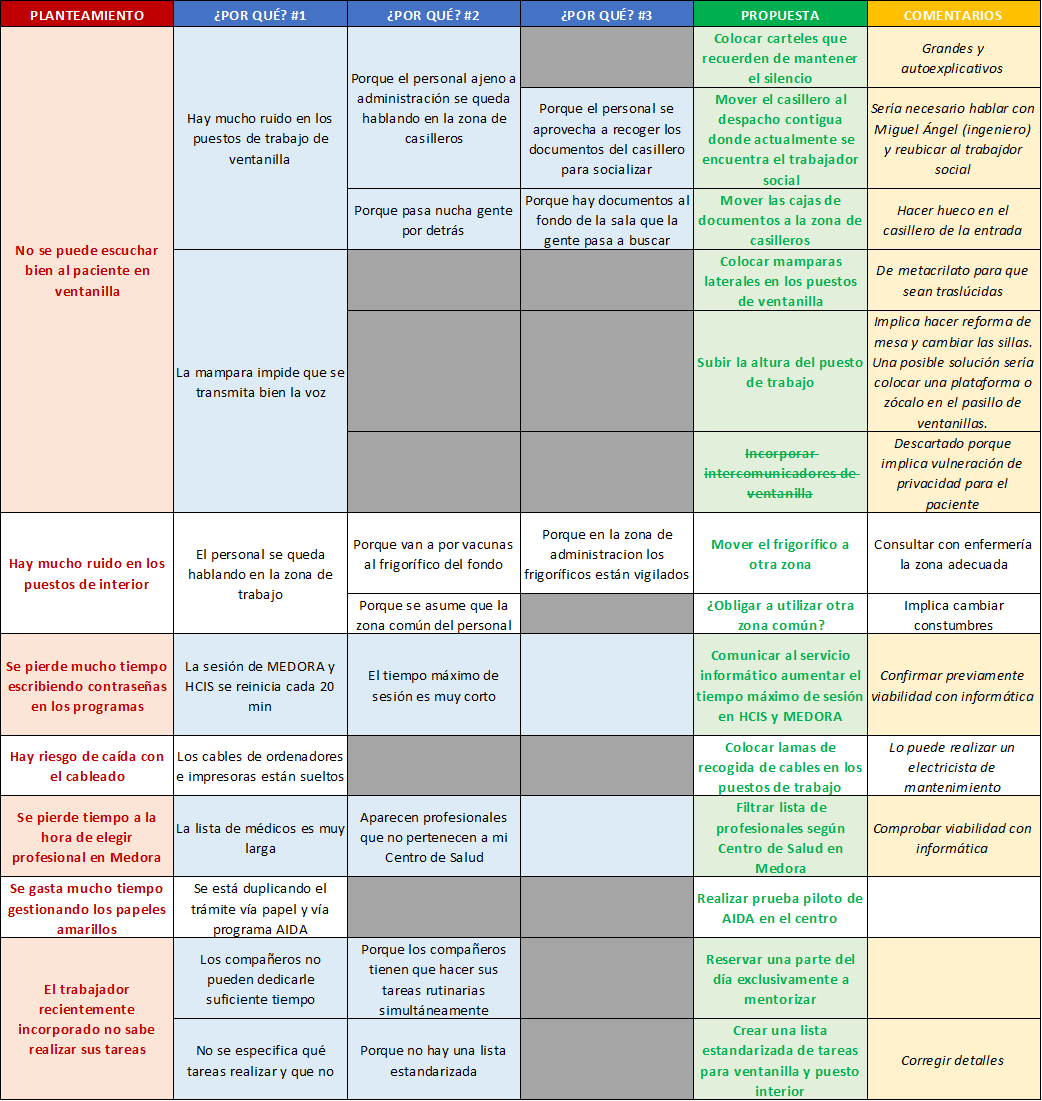
\includegraphics[width=\textwidth]{img/cinco-porques.png}
    \caption{Tabla de los cinco porqués}
    \label{fig:cinco-porques}
\end{figure}

\subsection{Comunicación complicada en ventanilla}

Los administrativos se quejan de que es difícil escuchar correctamente al pacientes al otro lado de la mampara.
Esto provoca que tengan que elevar la voz en numerosas ocasiones, lo que puede llegar a degenerar en problemas de salud.

Las causas son diversas, por un lado existe ruido ambiental en toda la zona interior de la oficina incluso estando separada del hall mediante una puerta.
Este ruido es debido al murmullo que se genera en la zona de los casilleros al concentrarse el gentío que va a recoger sus documentos.
También sucede que algunos de los documentos que no se encuentran en los casilleros, están al fondo de la sala de puestos de ventanilla lo que provoca que alguien que necesite de alguno de esos documentos se tenga que recorrer la sala pasando por detrás de los puestos.

A continuación se muestran las distintas propuestas de mejora que salieron en la reunión:

\begin{itemize}
    \item Colocar cartelería que recuerde mantener el silencio
    \item Mover el casillero al despacho contiguo
    \item Mover las cajas de documentos del fondo a los casilleros
    \item Colocar mamparas laterales en los puestos de ventanilla
    \item Subir la altura del puesto de trabajo
    \item Incorporar intercomunicadores de ventanilla
\end{itemize}

\subsection{Ruido ambiental en los puestos interiores}

En la zona interior de la sección administrativa, el personal se queja de que hay mucho ruido lo que les impide concentrarse en sus tareas laborales.
Esto es debido a que otros profesionales no administrativos lo utilizan como zona común para hablar entre ellos.
Además, muchas veces las enfermeras recorren toda la sala para recoger dosis de vacunas, ya que el frigorífico se encuentra en administración.

Algunas de las soluciones propuestas son las siguientes:

\begin{itemize}
    \item Informar al personal de que la zona de administración no es una sala de descanso
    \item Mover el frigorífico de las vacunas al sótano.
\end{itemize}

\subsection{El trabajador recién incorporado no tiene información}

Este es un problema común que existe en el ámbito sanitario debido a la alta rotación del personal.
Este problema está causado por una falta de tiempo y dedicación de los compañeros de trabajo al nuevo trabajador para enseñarle el funcionamiento de la sección administrativa. Es común que el trabajador veterano tenga que estar pendiente tanto de los usuarios de ventanilla como de las peticiones de los profesionales sanitarios. Esto hace que no se le pueda prestar la suficiente atención al trabajador nuevo y que su formación se alargue más de lo necesario.

Además, al trabajador recién incorporado no se le suele asignar tareas definidas y concretas sino que se espera de él que rinda plenamente desde el primer día asumiendo que posee todos los conocimientos necesarios. En parte, este problema surge de la ausencia de una lista de tareas estandarizadas, que es uno de los fines de este proyecto.

Entre las posibles mejoras propuestas se obtuvieron las siguientes:

\begin{itemize}
    \item Reservar una parte de la jornada exclusivamente a mentorizar al nuevo trabajador
    \item Crear una lista estandarizada de tareas para los puestos interiores y de ventanilla
\end{itemize}

\subsection{Gasto tiempo en escribir contraseñas}

Una queja común entre los administrativos es la gran cantidad de tiempo que pierden tecleando sus credenciales en los distintos programas informáticos sanitarios: \Gls{medora}, \Gls{hcis} o \Gls{tarjeta-sanitaria}.
Esto es debido a que las sesiones de los programas son muy cortas, entre 20 y 30 minutos, lo que se traduce entre 15 y 20 inicios de sesión por jornada.
En parte, esta mecánica fue diseñada para evitar que personas ajenas pudieran acceder al sistema en el caso de que el trabajador se olvidara de cerrar la sesión.

Un posible solución sería prolongar el tiempo máximo de sesión, pero no es sencillo ya que depende de servicios centrales y, en caso de realizar una modificación, habría que hacerla en todos y cada uno de los centros sanitarios de Castilla y León.

\subsection{Riesgo de caídas con el cableado}

Alrededor de las mesas de los puestos interiores se suelen acumular multitud de cables de pantallas, ordenadores o impresoras.
Se propone solicitar a mantenimiento colocar una lama que recoja todos los cables por los laterales de las mesas y así, evitar posibles caídas por tropiezo.

\subsection{Gasto de tiempo tramitando permisos}

Desde administración se quejan de que se pierde mucho tiempo tramitando los ``papeles amarillos'' ya que, aunque en los últimos años se ha implantado un programa informático para digitalizar el proceso, a día de hoy se está realizando la gestión por duplicado: vía digital y vía física.
Se plantea desde la Dirección de Gestión de Atención Primaria que el centro de salud de Laguna de Duero comience una prueba piloto con la nueva actualización del programa.
De esta forma los flujos de aprobación de los permisos retribuidos sería completamente digital.

\subsection{Analíticas no validadas}

Cuando un paciente llega a la ventanilla del centro con el volante para realizar una extracción de laboratorio, previamente el médico tiene que haber validado la analítica en el programa.
Si esto no ocurre, el administrativo tiene que buscar a un médico que valide la analítica en el momento ya que el paciente se encuentra a la espera de la prueba.
Esto genera una pérdida de tiempo considerable para el administrativo que prodría dedicarlo a otras tareas de mayor valor añadido.